\chapter{Introduzione}
\lecture{1}{07/10/2021}

L'obiettivo è quello di apprendere competenze in \textbf{tecnologie del vuoto} e \textbf{criogenia} in quanti questi due aspetti sono strettamente legati tra loro. Un classico esempio per cui si vuole introdurre l'apprendimento del vuoto e della criogenia è che i gradi di libertà quantistici sono fragili, soprattutto a variazioni termiche, queste vanno a distruggere la coerenza quantistica di uno stato quantistico, ad esempio un qubit. Questo comporta pertanto la perdita di informazioni e l'alterazione del nostro sistema.\\
Queste tecniche sono rilevanti nella fisica sperimentale perché danno accesso ad informazioni che normalmente non avremmo. In condizioni standard non avremmo accesso ad alcuni parametri.\\
Classici esempi di applicazioni sono ad esempio le misure di spettroscopia prossime allo zero assoluto, a queste temperature le righe spettrali sono più sottili e ciò comporta una risoluzione migliore.

\chapter{Tecnologie del vuoto}
Il \textbf{vuoto} è la condizione fisica che si realizza in un ambiente in cui la materia risulti prevalentemente allo stato gassoso e la pressione sia inferiore a quella atmosferica.

Come possiamo notare nel grafico RIFERIMENTO la pressione ha vari ordini di grandezza e delle regioni ben definite a seconda dell'intervallo di pressione che si vuole andare a realizzare. Proprio per quest'ultimo aspetto vi sono diversi dispositivi per realizzare tale un vuoto specifico. Uno dei problemi è che non esiste, attualmente, un unico dispositivo in grado di coprire tutte le condizioni di vuoto. Lo stesso discorso si applica per gli strumenti in grado di classificare il tipo di vuoto.

Il vuoto esiste in natura, oppure possiamo produrlo artificialmente per scopi scientifici. In natura lo lo abbiamo nello spazio e sulla superficie terrestre (la pressione tende a diminuire allontanandoci dall'atmosfera). Nello \textbf{spazio interstellare} non ha più senso parlare di pressione, in quanto si hanno davvero pochissime particelle, risulta quindi più opportuno parlare di densità di atomi o molecole. Lo stesso discorso a maggior ragione vale quando si considera lo \textbf{spazio intergalattico}.

\begin{center}
    \begin{tabular}{cc}
        \toprule
        Regione & Densità di particelle \\
        \midrule
        Spazio interstellare & $1 \frac{\text{atomo H}}{\text{cm}^3}$\\
        Spazio intergalattico & $ 1\frac{\text{atomo H}}{\text{mm}^3}$\\
        \bottomrule
    \end{tabular}\\
\end{center}

Come abbiamo detto, pompe diverse operano in regimi di vuoto diversi, quindi spesso sono usate pompe in serie così da ottenere pressioni $\tilde 10^{-11} \text{ mbar}$. Lo stesso discorso lo si applica ai dispositivi per classificare il tipo di vuoto.

Il vuoto è quindi un ambiente essenziale per gli esperimenti, questo è il motivo per cui la ISS (International Space Station) è in una regione ottimale del vuoto. Tuttavia non possiamo fare gran parte degli esperimenti là, ma bisogna farli sulla Terra creando il vuoto. Ad esempio al CERN, negli acceletori di particelle si hanno pressioni di $\tilde 10^{-11} \text{ mbar}$. Lo sviluppo di questo tipo di tecnologie è stata una conseguenza nel ricercare la costruzione ad esempio di acceleratori.

\begin{figure}[!ht]
    \centering
    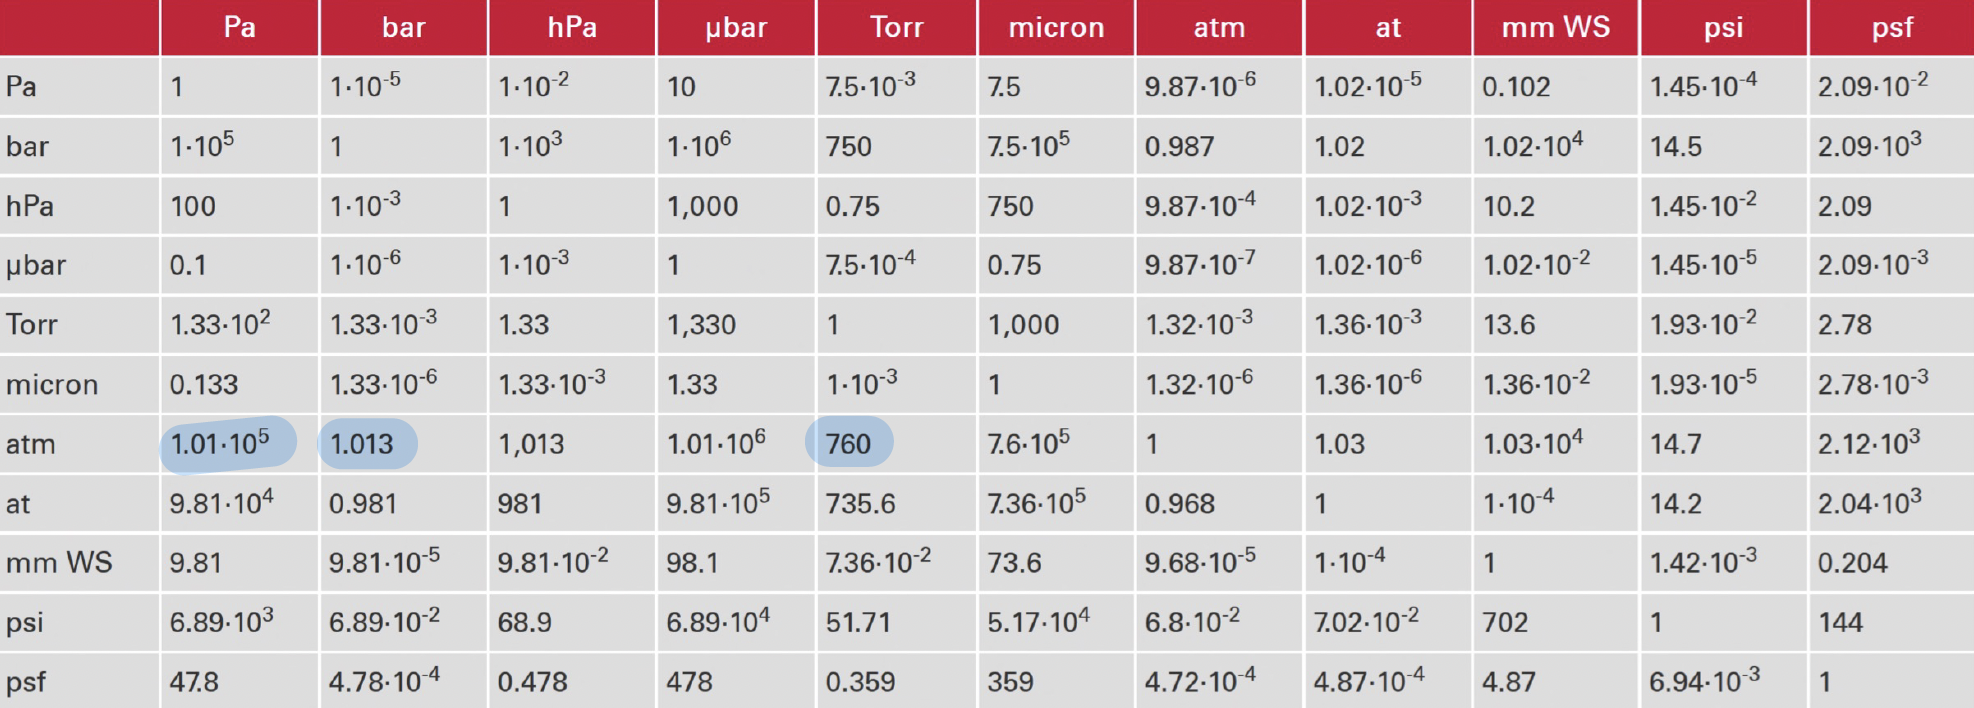
\includegraphics[scale=0.45]{images/pressuretablet.png}
\end{figure}

Il primo ciclotrone era una camera da vuoto da $10 \text{ cm}$ con pressioni nemmeno confrontambili con gli acceleratori attuali. Dal punto di vista storico si è passati da $10^{-5}-10^{-6} \text{ mbar}$ ai $10^{-11}-10^{-12} \text{ mbar}$.

\section{Perché si vuole produrre il vuoto?}
\begin{enumerate}
    \item Impedire processi di tipo chimico/fisico dovuti ai gas atmosferici. Ad esempio la fusione dei metalli reattivi come il titanio; oppure si vuole studiare la scarica di un gas;
    \item Accrescere il libero cammino medio delle particelle: effettuare un percorso senza che le particelle interagiscano con altre particelle non volute. Ad esempio negli acceleratori prima di entrare nella regione di collisione oppure nella fisica dei materiali per la deposizione dei film;
    \item Eliminare i gas che sono disciolti in un dato materiale o superficie. Dunque pulire superfici per la crescita di film nuovi oppure per il processo di liofilizzazione o rimorzione di oli da certi materiali;
    \item Ridurre la concentrazione di particolari gas sotto al livello critico. Ad esempio la scarica di un gas (un'applicazione ne è la televisione a tubo catodico);
    \item Simulare situazioni estreme. Ad esempio prima di mandare celle solari (o altri dispositivi) nello spazio per verificarne il funzionamento;
    \item Ridurre la frequenza delle collisioni con la superficie del nostro contenitore, abbatte la concentrazione delle superfici all'interno e migliora l'isolamento termico (in accordo con la criogenia).
\end{enumerate}

\subsection{Regimi di vuoto e applicazioni}

\begin{center}
    \begin{tabular}{*{15}{p{35mm}}}
        \toprule
        Regime di vuoto & Pa & mbar & Applicazioni \\
        \midrule
        Basso vuoto & $10^{5}-10^{2}$ & $10^3-1$ & Metallurgia (controllare acciai o scambi di calore tra due regioni). \\ \hline
        Vuoto medio & $10^{2}-10^{-1}$ & $1-10^{-3}$ & Industra alimentare per la liofilizzazione. \\ \hline
        Alto vuoto & $10^{-1}-10^{-6}$ & $10^{-3}-10^{-8}$ & Fisica dello stato solido: deposizione di film sottili o per esperimenti di tubi elettroni e alcuni rivelatori di fotoni e particelle. Fisica dei plasmi. \\ \hline
        Ultra alto vuoto & $< 10^{-6}$ & $< 10^{-8}$ & Fisica dello stato solido per lo studio delle superfici (no contaminazioni con altri notevoli) e negli acceleratori di particelle. \\
        \bottomrule
    \end{tabular}\\
\end{center}

\section{Cosa succede all'aria?}
Consideriamo l'aria come una miscela di diversi gas e utilizziamo la \textbf{legge di Dalton}:
\begin{equation*}
    P=\sum_i P_i
\end{equation*}

dove le $P_i$ rappresentano le pressioni parziali dell'i-esimo gas. In questo modo possiamo determinare l'effetto dei diversi atomi o molecole nel gas. Alcuni dispositivi possono selezionare la miscela da rimuovere durante il processo di creazione del vuoto. Non tutte le tecniche ovviamente hanno la stessa efficacia rispetto a tutti i tipi di gas, si deve quindi scegliere la tecnica giusta.

\begin{center}
    \begin{tabular}{ll}
        \toprule
        Componente & Pressione parziale ($\text{Pa}$) \\
        \midrule
        Azoto $\text{N}_2$ & $7.9104 \times 10^4$ \\
        Ossigeno $\text{O}_2$ & $ 2.1220 \times 10^4 $ \\
        Argon $\text{Ar}$ & $9.46 \times 10^2$ \\
        Biossido di carbonio $\text{CO}_2$ & $ 8.33 $\\
        Altri ($\text{He},\text{Ne}, \text{Kr}, \text{Xe}$) & $2$ \\
        \bottomrule
    \end{tabular} \\
\end{center}

Nei processi, l'elio e l'idrogeno essendo molto leggeri, sono i più difficili da eliminare e sono gli elementi più presenti nell'atmosfera della Luna.

Consideriamo il gas come un gas ideale, così da poter utilizzare l'equazione dei gas perfetti:
\begin{equation*}
    PV = nRT
\end{equation*}
Ricordando che:
\begin{equation*}
    n=\frac N {N_{\text A}} \ \ \ \ \ n=\frac{\text{massa}}{\text{peso atomico (g)}}=\frac{m}{A(g)} \ \ \ \ \ k_{\text B}=\frac{R}{N_{\text A}}
\end{equation*}
\begin{itemize}
    \item $N$: numero totale di particelle;
    \item $N_{\text A}$: numero di Avogadro ($6.022 \times 10^{23} \frac{\text{particelle}}{\text{mol}}$);
    \item $n$: numero di moli di una massa $m$ di sostanza di massa atomica $M$;
    \item $k_{\text B}$: costante di Boltzmann ($1.38 \times 10^{-23} \frac{\text J}{\text K}$);
    \item $R$: costante dei gas ($8.2\times 10^{-2} \frac{\text{atm L}}{\text{mol K}}$ oppure $8.31 \frac{\text{Pa m}^3}{\text{mol K}}$).
\end{itemize}
\begin{equation*}
    PV=Nk_{\text B}T
\end{equation*}
Possiamo esprimere il grado di vuoto come la densità di particelle $\frac NV=\frac{P}{k_{\text B}T}$ in $\text m^3$. Il significato fisico è quello di mantenere il volume costante e inserire un maggior numero di particelle cosicché aumenti la pressione, cioè una misura del numero di urti che le particelle hanno con le pareti. Questa riscrittura è utile perché permette di fare alcune considerazioni su alcuni casi specifici.

\begin{center}
    \begin{tabular}{ll}
        \toprule
        Regione & Densità di particelle \\
        \midrule
        Aria alla superficie terrestre & $\frac N V \sim 2\times10^{25}$ \\
        Atmosfera 10 km dalla superficie & $\frac N V \sim 4 \times10^{24}$ \\
        Atmosfera a 100 km dalla superficie & $\frac N V \sim 9 \times10^{18}$ \\
        Alto vuoto (in laboratorio) & $\frac N V \sim 3 \times10^{16}$ \\
        Atmosfera a 1000 km dalla superficie & $\frac N V \sim 5 \times 10^{13}$ \\
        Spazio interstellare & $\frac N V \sim 10^6$ \\
        Spazio intergalattico & $\frac N V \sim 1$ \\
        \bottomrule
    \end{tabular} \\
\end{center}

Se andiamo in una condizione di vuoto, meno particelle abbiamo, più la probabilità che una particella subisca un urto con un'altra particella diminuisce mentre il libero cammino medio aumenta.

\subsection{Libero cammino medio}
Definiamo il \textbf{libero cammino medio} come lo spazio percorso tra due urti successivi. Dalla teoria cinetica dei gas si ricava che:
\begin{equation*}
    \lambda = \frac{k_{\text B}T}{\sqrt 2 4 \pi r^2P}
\end{equation*}
In questo modello, si considera le particelle come sfere rigide dotate di un raggio $r \approx 10 \text{ nm}$. Osserviamo come $\lambda \propto \frac 1 P$, il che è ragionevole, perché per pressioni alte ho tante particelle che eseguiranno più urti tra loro e il libero cammino medio sarà piccolo.

[GRAFICO]

Il grafico è particolamente interessante:
\begin{itemize}
    \item Il libero cammino medio in alto vuoto ($P = 10^{-4}-10^{-1}$) è $ \lambda > 1 \text{ cm}$. Questa regione prende il nome di \textbf{vuoto molecolare}. Al di sotto di certi valori di pressioni il libero cammino medio può essere maggiore delle dimensioni del recipiente che contiene il gas. In questo caso prevalgono gli urti con le pareti e diventano importanti i fenomeni di interazione gas-solido. Il regime di alto o ultra alto vuoto è tipicamente usato per la deposizione di film sottili;
    \item Nella regione di basso vuoto abbiamo un libero cammino medio piccolo $\lambda \approx 10^{-6}-10^{-2}\text{ cm}$. Siamo nella condizione di \textbf{vuoto viscoso}. In questa regione prevalgono gli urti tra particelle che costituiscono il gas. Il gas è fatto da strati che possono scivolare gli uni sugli altri (esempio di fluido viscoso).
\end{itemize}
Questi aspetti sono da tenere in considerazione quando progetto una macchina da vuoto, in particolare eventuali interazioni con le superfici o le particelle del gas.

\section{Coesistenza di liquido/solido e vapore: tensione di vapore}
In alcuni regimi è importante l'interazione tra gas e liquido/solido. Se evaporazione e condensazione avvengono alla stessa velocità siamo in una condizione di equilibrio tra fase liquida/solida e quella gassosa. In particolar modo la pressione della fase gassosa viene detta \textbf{tensione di vapore}. È molto importante perché se abbiamo una condizione di evacuazione tra solido e gas avremo sempre una pressione che limiterà il vuoto minimo per realizzare il vuoto (pressione da raggiungere). Questo avviene tra la superficie del contenitore e il gas da evacuare.

Data una sostanza è data una legge che lega la temperatura alla tensione di vapore:
\begin{equation*}
    \log{P}=A-\frac{B}{T}+C\log{T}
\end{equation*}
dove $T$ è la temperatura e $A$, $B$ e $C$ sono delle costanti che dipendono dalla sostanza con cui abbiamo a che fare.
Questa relazione ci mostra che se la pressione è inferiore alla tensione di vapore ad una determinata temperatura, allora si ha il passaggio di particelle dalla fase condensata liquido/solido a quella gassosa e il processo andrà avanti finché non si raggiunge l'equilibrio. Possiamo sfruttare quindi la tecnologia del vuoto per utilizzare la pressione per favorire ad esempio il processo di crescita di un cristallo oppure usarlo nell'industria dei semiconduttori (transistor) oppure nei sistemi di qubit a superconduzione.

Il grafico [GRAFICO] mostra le curve di tensione di vapore di alcuni gas. I punti all'interno del grafico rappresentano i punti di fusione. Analizziamo ad esempio:
\begin{itemize}
    \item $\text{H}_2\text{O}$: ha un punto di fusione poco sotto i $300\text{ K}$ e la tensione di vapore a questa temperatura è inferiore a quella atmosferica: $P_\text{atm}>P_\text{vapore}$. Pertanto raffreddando il sistema a $0\text{\degree C}$ l'acqua passerà da vapore a solido/liquido. Invece a $100\text{\degree C}$ bolle e ho il passaggio da liquido a gas;
    \item $\text{N}_2$: ha un punto di fusione circa a $65\text{ K}$. A pressione atmosferica siamo a $T \sim 77\text{ K}$ per cui il liquido bolle. Se lo trovasiamo vediamo che bolle e una buona parte del gas esce. Non va tenuto in contenitori chiusi altrimenti esplodono. Il punto di transizione è a $\sim 36\text{ K}$, abbiamo quindi una transizione tra due fasi, dove l'azoto è solido e a $T < 36 \text{ K}$ cristallizza in fase $\alpha$ con reticolo FCC, mentre a $T > 36 \text{K}$ cristallizza in fase $\beta$ con reticolo esagonale.
\end{itemize}
Il comportamento dell'$\text{N}_2$ è analogo nello stagno in cui nella fase $\alpha$ è bianco e nella fase $\beta$ è grigio a $\sim 13\text{\degree C}$. Lo stagno nella fase $\beta$ è molto più fragile. La fase $\alpha$ invece è isolante topologicamente, posso realizzare un sistema per creare una separazione di spin e creare un sistema non dissipativo tra i portatori di carica per cui non possono fare scattering.
\section{Sistemi da vuoto}
[IMMAGINE]
Si tratta di una cavità che vogliamo evacuare equipaggiata con un misuratore di pressione e collegata con canalizzazioni alle pompe da vuoto che risucchiano il gas e lo espellono. La cavità è tipicamente in metallo (acciaio inossidabile per la crescita epiteliare) oppure in vetro. Lo sviluppo delle tecnologie per la realizzazione del vuoto è stato molto rapido, soprattutto negli ultimi anni, anche se la realizzazione di vuoto spinto risulta ancora difficile con un'unica pompa. Si hanno diverse pompe per i diversi regimi, quindi avremo diversi vantaggi e svantaggi per ognuna, soprattutto per quanto riguarda il gas residuo. La soluzione è quella di combinare più pompe da vuoto e quindi la pressione che si raggiunge dipende da molti fattori ad esempio la conduttanza dovuta a strozzature nella canalizzazione. Analizziamo i parametri del sistema da vuoto:
\begin{itemize}
    \item $V$: volume della cavità;
    \item $P_i$: pressione iniziale (solitamente è quella atmosferica) $P_{\text{atm}}\sim 760 \text{ torr}$;
    \item $P_f$: pressione finale che si vuole ottenere;
    \item $A$: superficie esposta al vuoto;
    \item $D$: tasso di degasaggio $\bigg[\frac{\text{torr L}}{{cm}^2\text{ s}}\bigg]$ collegata a $N\frac{PV}{k_\text{B}T}$, misura del numero di particelle che passano in fase gassosa dalle superficie del sistema da vuoto;
    \item $t$: tempo di evacuazione e dipende da alcuni parametri sperimentali tra cui:
    \item $s$: velocità di pompaggio ad una pressione data $\bigg[\frac{L}{s}\bigg]$
    \item $k$: portata $=P\times s$ $\bigg[\frac{\text{torr L}}{s}\bigg]$
\end{itemize}

L'equazione fondamentale che descrive questi problemi, valida su un intervallo di pressioni per cui la velocità di pompaggio è costante, è:
\begin{equation*}
    -\dv{PV}{t}=PS \Rightarrow \frac{\dd{P}}{P}=\frac s V \dd{t}
\end{equation*}
Risolvendo:
\begin{equation*}
    \ln{P}=-\frac{s}{V}t +{\text{cost}}
\end{equation*}
Integrando con le condizioni iniziali troviamo la costante:
\begin{equation*}
    s=\frac V t 2.3\bigg(\log{P_i}-\log{P_f}\bigg)
\end{equation*}
Definisce la pressione finale e quindi il tempo per raggiungere questa pressione finale.
Questo è importante per dimensionare il nostro sistema da vuoto. Precisiamo che $s$ non è costante, perché ogni pompa ha la sua velocità e un range di pressioni di utilizzo.
Esempio:

[GRAFICO]

\begin{itemize}
    \item Pompa per il regime viscoso;
    \item Pompa per il regime molecolare:
    \begin{equation*}
        P_f=\frac{AD}{s}
    \end{equation*} 
\end{itemize}
La pressione finale è limitata dal degasaggio, ovvero dal gas rilasciato dalle superficie. Questo se e solo se siamo in condizioni di assenza di perdite.